\section{Система с интервалом между наблюдениями}

Мы уже говорили, что реальные системы не могут передавать данные о своём положении непрерывно. В таком случае будем считать, что данные о состоянии передаются с некоторым известным (будем предполагать, детерминированным) интервалом времени. В таком случае можно рассматривать шаг сетки построенного алгоритма $\varepsilon$ как время между отправкой наблюдений. При этом мы не можем уменьшать шаг --- он становится фиксированным для рассматриваемой системы.

Как видно из рисунков Рис.~\ref{img:red-01} и Рис.~\ref{img:red-025}, построенные алгоритмом упраления приближают исходное в таком случае, но точность становится меньше. Зависимость среднеквадратичного отклонения функциона $J_\varepsilon$ от посчитанного без запаздывания $J$ приведена на рисунке Рис.~\ref{img:square}.

Особым случаем можно считать ситуацию, при которой время, между двумя отправками данных о состоянии $\varepsilon$ становится больше времени запаздывания $h$. В таком случае кажется естественным провести редукцию системы \eqref{eq:first_task} к дискретному виду.

Мы по прежнему строим кусочно-постоянное управление $u(t) = u^k$ на отрезке $t^{k+1} - h \leqslant t < t^{k+1} - h$. Обозначим за $x^{k} = x(t^k)$. Тогда применим формулу Коши:
\begin{multline*}
x^{k+1} = X(t^{k+1},\,t^k)x^k
+
\int\limits_{t^k}^{t^{k} + h} X(t^{k+1} - h,\,s)B(s)\,ds\cdot u^{k-1}
+\\+
\int\limits_{t^{k} + h}^{t^{k+1}} X(t^{k+1},\,s)B(s)\,ds\cdot u^{k}.
\end{multline*}
Из этого получаем следующую дискретную систему с запаздыванием по управлению:
\begin{equation}
        x^{k+1} = \Phi^k x^k + \Gamma_1^k u^{k} + \Gamma_2^k u^{k-1}.
\end{equation}






\tikzset{every picture/.style={line width=0.75pt}} %set default line width to 0.75pt        
\begin{figure}
\centering
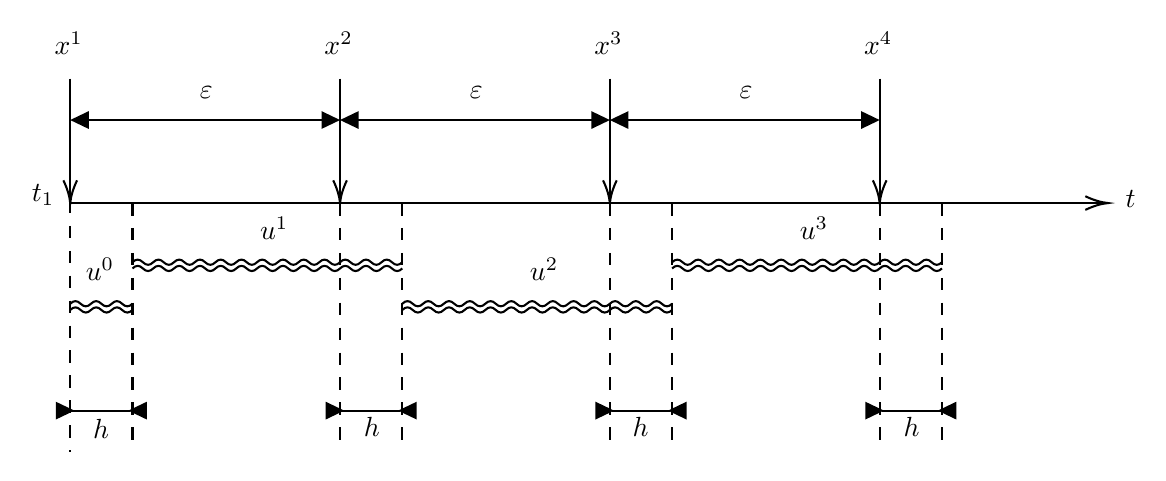
\begin{tikzpicture}[x=0.75pt,y=0.75pt,yscale=-1,xscale=1]
%uncomment if require: \path (0,300); %set diagram left start at 0, and has height of 300

%Straight Lines [id:da35985306918083526] 
\draw    (100,110) -- (598,110) ;
\draw [shift={(600,110)}, rotate = 180] [color={rgb, 255:red, 0; green, 0; blue, 0 }  ][line width=0.75]    (10.93,-3.29) .. controls (6.95,-1.4) and (3.31,-0.3) .. (0,0) .. controls (3.31,0.3) and (6.95,1.4) .. (10.93,3.29)   ;
%Straight Lines [id:da32106765450262065] 
\draw    (100,50) -- (100,108) ;
\draw [shift={(100,110)}, rotate = 270] [color={rgb, 255:red, 0; green, 0; blue, 0 }  ][line width=0.75]    (10.93,-3.29) .. controls (6.95,-1.4) and (3.31,-0.3) .. (0,0) .. controls (3.31,0.3) and (6.95,1.4) .. (10.93,3.29)   ;
%Straight Lines [id:da8214392914683835] 
\draw    (230,50) -- (230,108) ;
\draw [shift={(230,110)}, rotate = 270] [color={rgb, 255:red, 0; green, 0; blue, 0 }  ][line width=0.75]    (10.93,-3.29) .. controls (6.95,-1.4) and (3.31,-0.3) .. (0,0) .. controls (3.31,0.3) and (6.95,1.4) .. (10.93,3.29)   ;
%Straight Lines [id:da004791921615067252] 
\draw    (360,50) -- (360,108) ;
\draw [shift={(360,110)}, rotate = 270] [color={rgb, 255:red, 0; green, 0; blue, 0 }  ][line width=0.75]    (10.93,-3.29) .. controls (6.95,-1.4) and (3.31,-0.3) .. (0,0) .. controls (3.31,0.3) and (6.95,1.4) .. (10.93,3.29)   ;
%Straight Lines [id:da5712030850361053] 
\draw    (233,70) -- (357,70) ;
\draw [shift={(360,70)}, rotate = 180] [fill={rgb, 255:red, 0; green, 0; blue, 0 }  ][line width=0.08]  [draw opacity=0] (8.93,-4.29) -- (0,0) -- (8.93,4.29) -- cycle    ;
\draw [shift={(230,70)}, rotate = 0] [fill={rgb, 255:red, 0; green, 0; blue, 0 }  ][line width=0.08]  [draw opacity=0] (8.93,-4.29) -- (0,0) -- (8.93,4.29) -- cycle    ;
%Straight Lines [id:da9707227447008594] 
\draw  [dash pattern={on 4.5pt off 4.5pt}]  (100,109) -- (100,230) ;
%Straight Lines [id:da12490692567020634] 
\draw  [dash pattern={on 4.5pt off 4.5pt}]  (130,110) -- (130,230) ;
%Straight Lines [id:da24651362568684776] 
\draw  [dash pattern={on 4.5pt off 4.5pt}]  (230,110) -- (230,230) ;
%Straight Lines [id:da3268721449826282] 
\draw  [dash pattern={on 4.5pt off 4.5pt}]  (260,110) -- (260,230) ;
%Straight Lines [id:da8460646135972608] 
\draw  [dash pattern={on 4.5pt off 4.5pt}]  (360,110) -- (360,230) ;
%Straight Lines [id:da050181155508509545] 
\draw  [dash pattern={on 4.5pt off 4.5pt}]  (390,110) -- (390,230) ;
%Straight Lines [id:da40778935140992556] 
\draw    (101,210) -- (129,210) ;
\draw [shift={(128,210)}, rotate = 0] [fill={rgb, 255:red, 0; green, 0; blue, 0 }  ][line width=0.08]  [draw opacity=0] (8.93,-4.29) -- (0,0) -- (8.93,4.29) -- cycle    ;
\draw [shift={(102,210)}, rotate = 180] [fill={rgb, 255:red, 0; green, 0; blue, 0 }  ][line width=0.08]  [draw opacity=0] (8.93,-4.29) -- (0,0) -- (8.93,4.29) -- cycle    ;
%Straight Lines [id:da25231316824794214] 
\draw    (231,210) -- (259,210) ;
\draw [shift={(258,210)}, rotate = 0] [fill={rgb, 255:red, 0; green, 0; blue, 0 }  ][line width=0.08]  [draw opacity=0] (8.93,-4.29) -- (0,0) -- (8.93,4.29) -- cycle    ;
\draw [shift={(232,210)}, rotate = 180] [fill={rgb, 255:red, 0; green, 0; blue, 0 }  ][line width=0.08]  [draw opacity=0] (8.93,-4.29) -- (0,0) -- (8.93,4.29) -- cycle    ;
%Straight Lines [id:da7485299203870347] 
\draw    (361,210) -- (389,210) ;
\draw [shift={(388,210)}, rotate = 0] [fill={rgb, 255:red, 0; green, 0; blue, 0 }  ][line width=0.08]  [draw opacity=0] (8.93,-4.29) -- (0,0) -- (8.93,4.29) -- cycle    ;
\draw [shift={(362,210)}, rotate = 180] [fill={rgb, 255:red, 0; green, 0; blue, 0 }  ][line width=0.08]  [draw opacity=0] (8.93,-4.29) -- (0,0) -- (8.93,4.29) -- cycle    ;
%Straight Lines [id:da6433056942372144] 
\draw    (130,138.5) .. controls (131.67,136.83) and (133.33,136.83) .. (135,138.5) .. controls (136.67,140.17) and (138.33,140.17) .. (140,138.5) .. controls (141.67,136.83) and (143.33,136.83) .. (145,138.5) .. controls (146.67,140.17) and (148.33,140.17) .. (150,138.5) .. controls (151.67,136.83) and (153.33,136.83) .. (155,138.5) .. controls (156.67,140.17) and (158.33,140.17) .. (160,138.5) .. controls (161.67,136.83) and (163.33,136.83) .. (165,138.5) .. controls (166.67,140.17) and (168.33,140.17) .. (170,138.5) .. controls (171.67,136.83) and (173.33,136.83) .. (175,138.5) .. controls (176.67,140.17) and (178.33,140.17) .. (180,138.5) .. controls (181.67,136.83) and (183.33,136.83) .. (185,138.5) .. controls (186.67,140.17) and (188.33,140.17) .. (190,138.5) .. controls (191.67,136.83) and (193.33,136.83) .. (195,138.5) .. controls (196.67,140.17) and (198.33,140.17) .. (200,138.5) .. controls (201.67,136.83) and (203.33,136.83) .. (205,138.5) .. controls (206.67,140.17) and (208.33,140.17) .. (210,138.5) .. controls (211.67,136.83) and (213.33,136.83) .. (215,138.5) .. controls (216.67,140.17) and (218.33,140.17) .. (220,138.5) .. controls (221.67,136.83) and (223.33,136.83) .. (225,138.5) .. controls (226.67,140.17) and (228.33,140.17) .. (230,138.5) .. controls (231.67,136.83) and (233.33,136.83) .. (235,138.5) .. controls (236.67,140.17) and (238.33,140.17) .. (240,138.5) .. controls (241.67,136.83) and (243.33,136.83) .. (245,138.5) .. controls (246.67,140.17) and (248.33,140.17) .. (250,138.5) .. controls (251.67,136.83) and (253.33,136.83) .. (255,138.5) .. controls (256.67,140.17) and (258.33,140.17) .. (260,138.5) -- (260,138.5)(130,141.5) .. controls (131.67,139.83) and (133.33,139.83) .. (135,141.5) .. controls (136.67,143.17) and (138.33,143.17) .. (140,141.5) .. controls (141.67,139.83) and (143.33,139.83) .. (145,141.5) .. controls (146.67,143.17) and (148.33,143.17) .. (150,141.5) .. controls (151.67,139.83) and (153.33,139.83) .. (155,141.5) .. controls (156.67,143.17) and (158.33,143.17) .. (160,141.5) .. controls (161.67,139.83) and (163.33,139.83) .. (165,141.5) .. controls (166.67,143.17) and (168.33,143.17) .. (170,141.5) .. controls (171.67,139.83) and (173.33,139.83) .. (175,141.5) .. controls (176.67,143.17) and (178.33,143.17) .. (180,141.5) .. controls (181.67,139.83) and (183.33,139.83) .. (185,141.5) .. controls (186.67,143.17) and (188.33,143.17) .. (190,141.5) .. controls (191.67,139.83) and (193.33,139.83) .. (195,141.5) .. controls (196.67,143.17) and (198.33,143.17) .. (200,141.5) .. controls (201.67,139.83) and (203.33,139.83) .. (205,141.5) .. controls (206.67,143.17) and (208.33,143.17) .. (210,141.5) .. controls (211.67,139.83) and (213.33,139.83) .. (215,141.5) .. controls (216.67,143.17) and (218.33,143.17) .. (220,141.5) .. controls (221.67,139.83) and (223.33,139.83) .. (225,141.5) .. controls (226.67,143.17) and (228.33,143.17) .. (230,141.5) .. controls (231.67,139.83) and (233.33,139.83) .. (235,141.5) .. controls (236.67,143.17) and (238.33,143.17) .. (240,141.5) .. controls (241.67,139.83) and (243.33,139.83) .. (245,141.5) .. controls (246.67,143.17) and (248.33,143.17) .. (250,141.5) .. controls (251.67,139.83) and (253.33,139.83) .. (255,141.5) .. controls (256.67,143.17) and (258.33,143.17) .. (260,141.5) -- (260,141.5) ;
%Straight Lines [id:da43614197953958656] 
\draw    (100,158.5) .. controls (101.67,156.83) and (103.33,156.83) .. (105,158.5) .. controls (106.67,160.17) and (108.33,160.17) .. (110,158.5) .. controls (111.67,156.83) and (113.33,156.83) .. (115,158.5) .. controls (116.67,160.17) and (118.33,160.17) .. (120,158.5) .. controls (121.67,156.83) and (123.33,156.83) .. (125,158.5) .. controls (126.67,160.17) and (128.33,160.17) .. (130,158.5) -- (130,158.5)(100,161.5) .. controls (101.67,159.83) and (103.33,159.83) .. (105,161.5) .. controls (106.67,163.17) and (108.33,163.17) .. (110,161.5) .. controls (111.67,159.83) and (113.33,159.83) .. (115,161.5) .. controls (116.67,163.17) and (118.33,163.17) .. (120,161.5) .. controls (121.67,159.83) and (123.33,159.83) .. (125,161.5) .. controls (126.67,163.17) and (128.33,163.17) .. (130,161.5) -- (130,161.5) ;
%Straight Lines [id:da5166290012929178] 
\draw    (260,158.5) .. controls (261.67,156.83) and (263.33,156.83) .. (265,158.5) .. controls (266.67,160.17) and (268.33,160.17) .. (270,158.5) .. controls (271.67,156.83) and (273.33,156.83) .. (275,158.5) .. controls (276.67,160.17) and (278.33,160.17) .. (280,158.5) .. controls (281.67,156.83) and (283.33,156.83) .. (285,158.5) .. controls (286.67,160.17) and (288.33,160.17) .. (290,158.5) .. controls (291.67,156.83) and (293.33,156.83) .. (295,158.5) .. controls (296.67,160.17) and (298.33,160.17) .. (300,158.5) .. controls (301.67,156.83) and (303.33,156.83) .. (305,158.5) .. controls (306.67,160.17) and (308.33,160.17) .. (310,158.5) .. controls (311.67,156.83) and (313.33,156.83) .. (315,158.5) .. controls (316.67,160.17) and (318.33,160.17) .. (320,158.5) .. controls (321.67,156.83) and (323.33,156.83) .. (325,158.5) .. controls (326.67,160.17) and (328.33,160.17) .. (330,158.5) .. controls (331.67,156.83) and (333.33,156.83) .. (335,158.5) .. controls (336.67,160.17) and (338.33,160.17) .. (340,158.5) .. controls (341.67,156.83) and (343.33,156.83) .. (345,158.5) .. controls (346.67,160.17) and (348.33,160.17) .. (350,158.5) .. controls (351.67,156.83) and (353.33,156.83) .. (355,158.5) .. controls (356.67,160.17) and (358.33,160.17) .. (360,158.5) .. controls (361.67,156.83) and (363.33,156.83) .. (365,158.5) .. controls (366.67,160.17) and (368.33,160.17) .. (370,158.5) .. controls (371.67,156.83) and (373.33,156.83) .. (375,158.5) .. controls (376.67,160.17) and (378.33,160.17) .. (380,158.5) .. controls (381.67,156.83) and (383.33,156.83) .. (385,158.5) .. controls (386.67,160.17) and (388.33,160.17) .. (390,158.5) -- (390,158.5)(260,161.5) .. controls (261.67,159.83) and (263.33,159.83) .. (265,161.5) .. controls (266.67,163.17) and (268.33,163.17) .. (270,161.5) .. controls (271.67,159.83) and (273.33,159.83) .. (275,161.5) .. controls (276.67,163.17) and (278.33,163.17) .. (280,161.5) .. controls (281.67,159.83) and (283.33,159.83) .. (285,161.5) .. controls (286.67,163.17) and (288.33,163.17) .. (290,161.5) .. controls (291.67,159.83) and (293.33,159.83) .. (295,161.5) .. controls (296.67,163.17) and (298.33,163.17) .. (300,161.5) .. controls (301.67,159.83) and (303.33,159.83) .. (305,161.5) .. controls (306.67,163.17) and (308.33,163.17) .. (310,161.5) .. controls (311.67,159.83) and (313.33,159.83) .. (315,161.5) .. controls (316.67,163.17) and (318.33,163.17) .. (320,161.5) .. controls (321.67,159.83) and (323.33,159.83) .. (325,161.5) .. controls (326.67,163.17) and (328.33,163.17) .. (330,161.5) .. controls (331.67,159.83) and (333.33,159.83) .. (335,161.5) .. controls (336.67,163.17) and (338.33,163.17) .. (340,161.5) .. controls (341.67,159.83) and (343.33,159.83) .. (345,161.5) .. controls (346.67,163.17) and (348.33,163.17) .. (350,161.5) .. controls (351.67,159.83) and (353.33,159.83) .. (355,161.5) .. controls (356.67,163.17) and (358.33,163.17) .. (360,161.5) .. controls (361.67,159.83) and (363.33,159.83) .. (365,161.5) .. controls (366.67,163.17) and (368.33,163.17) .. (370,161.5) .. controls (371.67,159.83) and (373.33,159.83) .. (375,161.5) .. controls (376.67,163.17) and (378.33,163.17) .. (380,161.5) .. controls (381.67,159.83) and (383.33,159.83) .. (385,161.5) .. controls (386.67,163.17) and (388.33,163.17) .. (390,161.5) -- (390,161.5) ;
%Straight Lines [id:da7310536979710727] 
\draw    (490,50) -- (490,108) ;
\draw [shift={(490,110)}, rotate = 270] [color={rgb, 255:red, 0; green, 0; blue, 0 }  ][line width=0.75]    (10.93,-3.29) .. controls (6.95,-1.4) and (3.31,-0.3) .. (0,0) .. controls (3.31,0.3) and (6.95,1.4) .. (10.93,3.29)   ;
%Straight Lines [id:da12502452123196184] 
\draw    (363,70) -- (487,70) ;
\draw [shift={(490,70)}, rotate = 180] [fill={rgb, 255:red, 0; green, 0; blue, 0 }  ][line width=0.08]  [draw opacity=0] (8.93,-4.29) -- (0,0) -- (8.93,4.29) -- cycle    ;
\draw [shift={(360,70)}, rotate = 0] [fill={rgb, 255:red, 0; green, 0; blue, 0 }  ][line width=0.08]  [draw opacity=0] (8.93,-4.29) -- (0,0) -- (8.93,4.29) -- cycle    ;
%Straight Lines [id:da567384646470296] 
\draw  [dash pattern={on 4.5pt off 4.5pt}]  (490,110) -- (490,230) ;
%Straight Lines [id:da9393775253321939] 
\draw  [dash pattern={on 4.5pt off 4.5pt}]  (520,110) -- (520,230) ;
%Straight Lines [id:da5549100836347505] 
\draw    (491,210) -- (519,210) ;
\draw [shift={(518,210)}, rotate = 0] [fill={rgb, 255:red, 0; green, 0; blue, 0 }  ][line width=0.08]  [draw opacity=0] (8.93,-4.29) -- (0,0) -- (8.93,4.29) -- cycle    ;
\draw [shift={(492,210)}, rotate = 180] [fill={rgb, 255:red, 0; green, 0; blue, 0 }  ][line width=0.08]  [draw opacity=0] (8.93,-4.29) -- (0,0) -- (8.93,4.29) -- cycle    ;
%Straight Lines [id:da3553751948082903] 
\draw    (390,138.5) .. controls (391.67,136.83) and (393.33,136.83) .. (395,138.5) .. controls (396.67,140.17) and (398.33,140.17) .. (400,138.5) .. controls (401.67,136.83) and (403.33,136.83) .. (405,138.5) .. controls (406.67,140.17) and (408.33,140.17) .. (410,138.5) .. controls (411.67,136.83) and (413.33,136.83) .. (415,138.5) .. controls (416.67,140.17) and (418.33,140.17) .. (420,138.5) .. controls (421.67,136.83) and (423.33,136.83) .. (425,138.5) .. controls (426.67,140.17) and (428.33,140.17) .. (430,138.5) .. controls (431.67,136.83) and (433.33,136.83) .. (435,138.5) .. controls (436.67,140.17) and (438.33,140.17) .. (440,138.5) .. controls (441.67,136.83) and (443.33,136.83) .. (445,138.5) .. controls (446.67,140.17) and (448.33,140.17) .. (450,138.5) .. controls (451.67,136.83) and (453.33,136.83) .. (455,138.5) .. controls (456.67,140.17) and (458.33,140.17) .. (460,138.5) .. controls (461.67,136.83) and (463.33,136.83) .. (465,138.5) .. controls (466.67,140.17) and (468.33,140.17) .. (470,138.5) .. controls (471.67,136.83) and (473.33,136.83) .. (475,138.5) .. controls (476.67,140.17) and (478.33,140.17) .. (480,138.5) .. controls (481.67,136.83) and (483.33,136.83) .. (485,138.5) .. controls (486.67,140.17) and (488.33,140.17) .. (490,138.5) .. controls (491.67,136.83) and (493.33,136.83) .. (495,138.5) .. controls (496.67,140.17) and (498.33,140.17) .. (500,138.5) .. controls (501.67,136.83) and (503.33,136.83) .. (505,138.5) .. controls (506.67,140.17) and (508.33,140.17) .. (510,138.5) .. controls (511.67,136.83) and (513.33,136.83) .. (515,138.5) .. controls (516.67,140.17) and (518.33,140.17) .. (520,138.5) -- (520,138.5)(390,141.5) .. controls (391.67,139.83) and (393.33,139.83) .. (395,141.5) .. controls (396.67,143.17) and (398.33,143.17) .. (400,141.5) .. controls (401.67,139.83) and (403.33,139.83) .. (405,141.5) .. controls (406.67,143.17) and (408.33,143.17) .. (410,141.5) .. controls (411.67,139.83) and (413.33,139.83) .. (415,141.5) .. controls (416.67,143.17) and (418.33,143.17) .. (420,141.5) .. controls (421.67,139.83) and (423.33,139.83) .. (425,141.5) .. controls (426.67,143.17) and (428.33,143.17) .. (430,141.5) .. controls (431.67,139.83) and (433.33,139.83) .. (435,141.5) .. controls (436.67,143.17) and (438.33,143.17) .. (440,141.5) .. controls (441.67,139.83) and (443.33,139.83) .. (445,141.5) .. controls (446.67,143.17) and (448.33,143.17) .. (450,141.5) .. controls (451.67,139.83) and (453.33,139.83) .. (455,141.5) .. controls (456.67,143.17) and (458.33,143.17) .. (460,141.5) .. controls (461.67,139.83) and (463.33,139.83) .. (465,141.5) .. controls (466.67,143.17) and (468.33,143.17) .. (470,141.5) .. controls (471.67,139.83) and (473.33,139.83) .. (475,141.5) .. controls (476.67,143.17) and (478.33,143.17) .. (480,141.5) .. controls (481.67,139.83) and (483.33,139.83) .. (485,141.5) .. controls (486.67,143.17) and (488.33,143.17) .. (490,141.5) .. controls (491.67,139.83) and (493.33,139.83) .. (495,141.5) .. controls (496.67,143.17) and (498.33,143.17) .. (500,141.5) .. controls (501.67,139.83) and (503.33,139.83) .. (505,141.5) .. controls (506.67,143.17) and (508.33,143.17) .. (510,141.5) .. controls (511.67,139.83) and (513.33,139.83) .. (515,141.5) .. controls (516.67,143.17) and (518.33,143.17) .. (520,141.5) -- (520,141.5) ;
%Straight Lines [id:da76267213163528] 
\draw    (103,70) -- (227,70) ;
\draw [shift={(230,70)}, rotate = 180] [fill={rgb, 255:red, 0; green, 0; blue, 0 }  ][line width=0.08]  [draw opacity=0] (8.93,-4.29) -- (0,0) -- (8.93,4.29) -- cycle    ;
\draw [shift={(100,70)}, rotate = 0] [fill={rgb, 255:red, 0; green, 0; blue, 0 }  ][line width=0.08]  [draw opacity=0] (8.93,-4.29) -- (0,0) -- (8.93,4.29) -- cycle    ;

% Text Node
\draw (91,26) node [anchor=north west][inner sep=0.75pt]    {$x^{1}$};
% Text Node
\draw (221,26) node [anchor=north west][inner sep=0.75pt]    {$x^{2}$};
% Text Node
\draw (351,26) node [anchor=north west][inner sep=0.75pt]    {$x^{3}$};
% Text Node
\draw (161,52.4) node [anchor=north west][inner sep=0.75pt]    {$\varepsilon $};
% Text Node
\draw (291,52.4) node [anchor=north west][inner sep=0.75pt]    {$\varepsilon $};
% Text Node
\draw (109.5,212.9) node [anchor=north west][inner sep=0.75pt]    {$h$};
% Text Node
\draw (240,211.9) node [anchor=north west][inner sep=0.75pt]    {$h$};
% Text Node
\draw (369.5,211.9) node [anchor=north west][inner sep=0.75pt]    {$h$};
% Text Node
\draw (481,26) node [anchor=north west][inner sep=0.75pt]    {$x^{4}$};
% Text Node
\draw (421,52.4) node [anchor=north west][inner sep=0.75pt]    {$\varepsilon $};
% Text Node
\draw (500,211.9) node [anchor=north west][inner sep=0.75pt]    {$h$};
% Text Node
\draw (106,135) node [anchor=north west][inner sep=0.75pt]    {$u^{0}$};
% Text Node
\draw (190,115) node [anchor=north west][inner sep=0.75pt]    {$u^{1}$};
% Text Node
\draw (320,135) node [anchor=north west][inner sep=0.75pt]    {$u^{2}$};
% Text Node
\draw (450,115) node [anchor=north west][inner sep=0.75pt]    {$u^{3}$};
% Text Node
\draw (551,52.4) node [anchor=north west][inner sep=0.75pt]    {$\dotsc $};
% Text Node
\draw (551,142.4) node [anchor=north west][inner sep=0.75pt]    {$\dotsc $};
% Text Node
\draw (607,102.4) node [anchor=north west][inner sep=0.75pt]    {$t$};
% Text Node
\draw (80,99.4) node [anchor=north west][inner sep=0.75pt]    {$t_{1}$};


\end{tikzpicture}
\caption{Иллюстрация системы, где величина запаздывания $h$ меньше интервала времени между наблюдениями $\varepsilon$. Здесь показано в какие моменты времени наблюдается состояние системы и на каких промежутках действуют постоянные управления.}
\end{figure}


\begin{figure}[bh]
        \noindent\centering{
        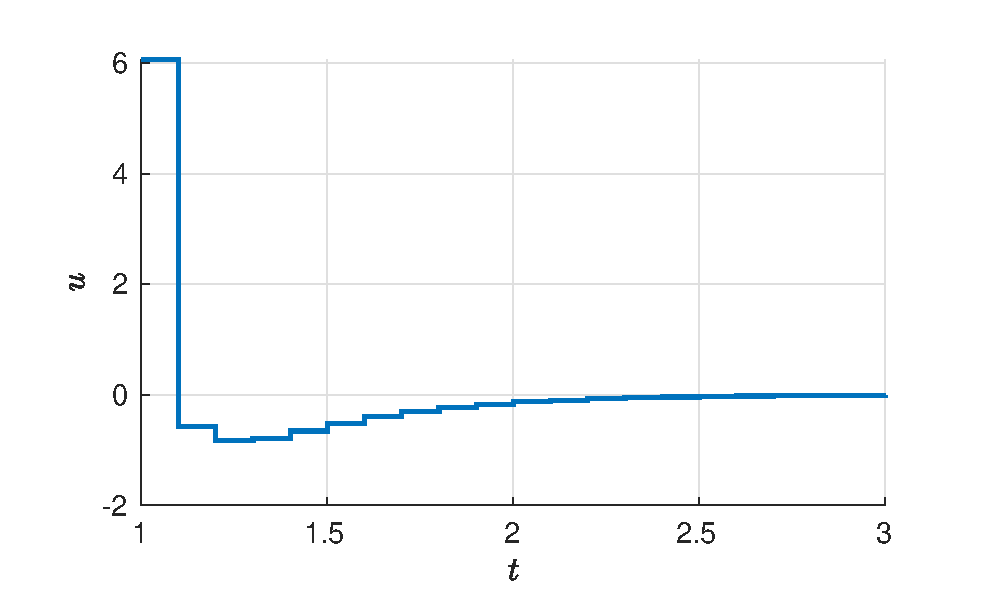
\includegraphics[width=160mm]{content/reduction/01.eps}
        }
        \caption{Оптимальная стратегия с запаздыванием наблюдения $h = 0,\!5$ для системы~\eqref{eq:x-example} с разбиением $\varepsilon = 0,\!1$.}
        \label{img:red-01}
\end{figure}
\begin{figure}[bh]
        \noindent\centering{
        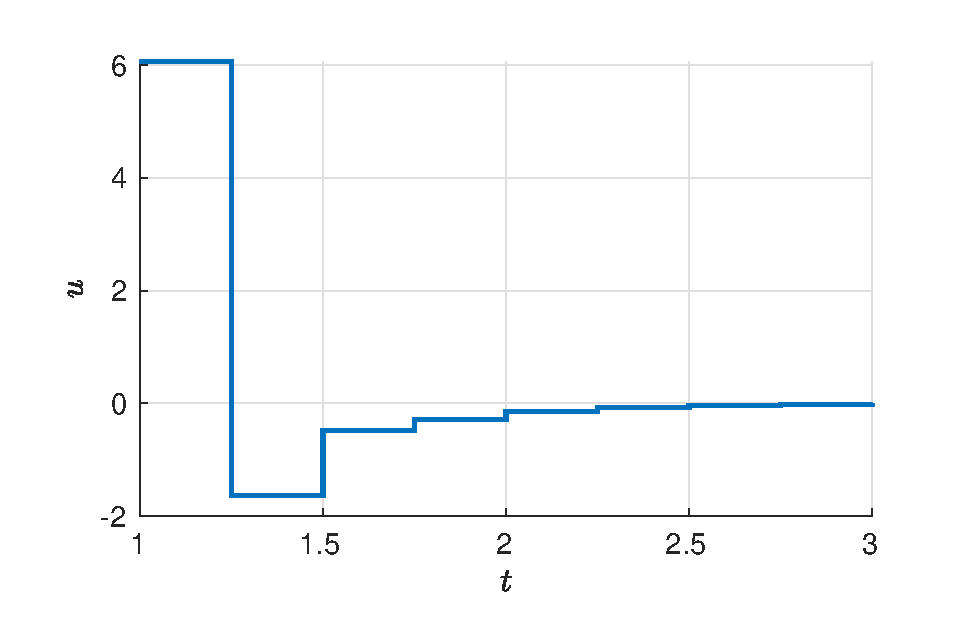
\includegraphics[width=160mm]{content/reduction/025.eps}
        }
        \caption{Оптимальная стратегия с запаздыванием наблюдения $h = 0,\!5$ для системы~\eqref{eq:x-example} с разбиением $\varepsilon = 0,\!25$.}
        \label{img:red-025}
\end{figure}
\begin{figure}[bh]
        \noindent\centering{
        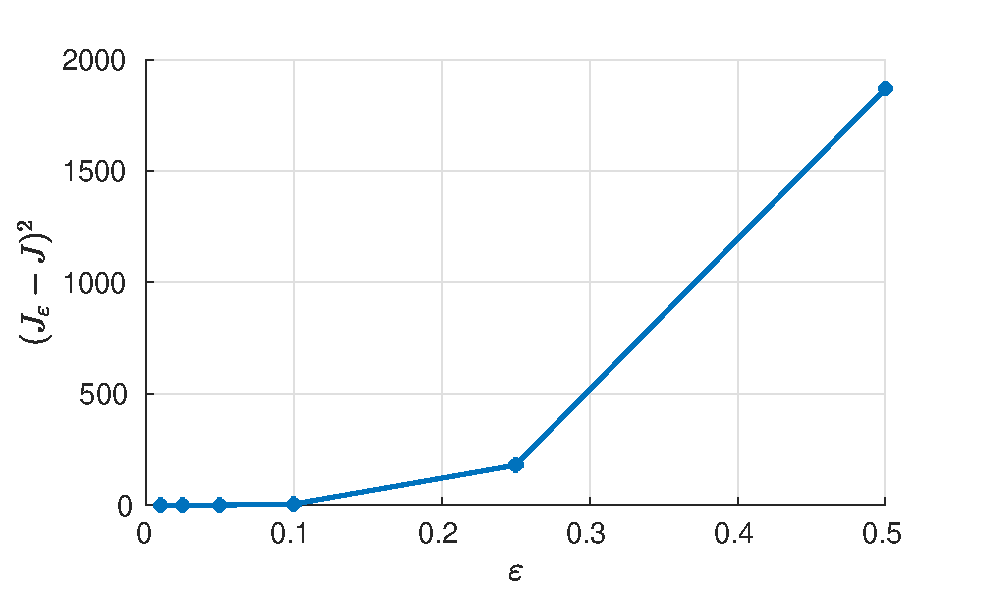
\includegraphics[width=160mm]{content/reduction/square.eps}
        }
        \caption{Среднеквадратичное отклонение функционала качества построенного алгоритма в зависимости от шага сетки $\varepsilon$. Здесь время запаздывания выбрано $h = 0,\!5$.}
        \label{img:square}
\end{figure}